\documentclass{beamer}

\mode<presentation>
{
  \usetheme{default}     
  \usecolortheme{default} 
  \usefonttheme{default} 
  \setbeamertemplate{navigation symbols}{}
  \setbeamertemplate{caption}[numbered]
} 

\usepackage[french]{babel}

\title[Cognition Informatique]{Modélisation Informatique de la Cognition}
\author{Kaan ERASLAN \and François JOUEN}
\institute{EPHE - PSL}
\date{\today}

\begin{document}

\begin{frame}
  \titlepage
\end{frame}

%\begin{frame}{Outline}
%  \tableofcontents
%\end{frame}

\section{Définition}

\begin{frame}{Cognition Naturelle}
\begin{columns}
\begin{column}{.5\textwidth}
     \begin{block}{}
     La \textbf{cognition} est un terme générique qui sert à désigner l'ensemble des processus mentaux qui se rapportent à la connaissance tels que:
\begin{itemize}
  \item Intelligence
  \item mémoire
  \item langage
  \item raisonnement
  \item prise de décision
  \item ...
\end{itemize}

    \end{block}
    \end{column}
    \begin{column}{.5\textwidth}
    \begin{block}{}

    \includegraphics[width=\textwidth]{cognitionNaturelle.png}
    \end{block}
    \end{column}
\end{columns}
\end{frame}

\begin{frame}{Définition Incomplète}
\begin{itemize}
    \item Idée implicite d’un dualisme corps/esprit
    \item Hiérarchisation avec l’idée de processus plus élémentaires (de bas niveau) comme la perception, la motricité ou encore les émotions
    \item Accent mis sur  les processus de traitement de l'information (de haut niveau) qui seraient les seuls dignes d’intérêt
    \item C’est oublier que les fonctions exécutives associent des processus de bas niveau et de haut niveau
\end{itemize}
\end{frame}

\begin{frame}{Une définition minimaliste}

Cognition est:
\begin{itemize}
    \item La capacité d’un système à intégrer à son fonctionnement les effets de l’environnement en réponse à sa propre activité.
    \item Approche centrée sur l’interaction système environnement
    \item Approche sensori-motrice
\end{itemize}
    
\end{frame}

\section{Environnement/Milieu}

\begin{frame}{La nécessaire distinction environnement/milieu}
\begin{columns}
\begin{column}{.7\textwidth}
     \begin{block}{}
\begin{itemize}
  \item \textbf{environnement} et \textbf{milieu}
  \item L’environnement se définit par l’existence de constantes physiques (la pesanteur, la vitesse de la lumière …)
  \item Le milieu: un certain environnement, spécifiquement approprié par les mécanismes cognitifs de cette espèce (ou de cette culture)
  
\end{itemize}
\end{block}
\end{column}
\begin{column}{.4\textwidth}
\begin{block}{}
    \includegraphics[width=\textwidth]{milieu01.png}
    \end{block}
    \end{column}
\end{columns}
\end{frame}
\note[itemize]{
\item \textbf{environnement} et \textbf{milieu}: \textbf{Toute cognition s’exerce dans un environnement}, mais il est nécessaire de faire une distinction entre
\item constantes physiques (la pesanteur, la vitesse de la lumière …)
\item Le milieu désigne la réalité physique de l’environnement pour une espèce (ou une culture) donnée,un certain environnement, spécifiquement approprié par les mécanismes cognitifs de cette espèce (ou de cette culture)
}

\section{Cognition Naturelle}

\begin{frame}{Notre cognition (naturelle) est épigénétique !}
\begin{figure}
    \centering
    \includegraphics[width=\textwidth]{epigeneticScheme.png}
    \caption{Travaux de Gotlieb}
    \label{fig:my_label}
\end{figure}{}
    
\end{frame}

\begin{frame}{Formation des Neurons dans l'Espèce}
\begin{columns}
\begin{column}{0.7\textwidth}
\begin{block}{}
La neurogenèse \textbf{dépend de l’expérience}:
\begin{itemize}
    \item La neurogénèse repose sur l’ensemble des processus cellulaires qui permettent la mise en place de notre neuro anatomie.
    \item La neurogenèse est un système dépendant d’expériences (ex: induction cellulaire et fenêtres temporelles).
    \item Ensemble de neurones dont chacun apparaît comme une entité originale qui se distingue des autres par sa forme et le nombre de ses connexions.
    \item Commun à tous les membres d’une espèce donnée
\end{itemize}
\end{block}
\end{column}
\begin{column}{0.3\textwidth}
\begin{block}{}
\begin{figure}
    \centering
    \includegraphics[width=\textwidth]{neuroGenesis01.png}
    \caption{Neuron}
    \label{fig:my_label}
\end{figure}
\end{block}
\end{column}
\end{columns}
\end{frame}
\note[itemize]{
\item Processus cellulaires (multiplication, migration, différenciation, apoptose, myélinogenèse, et corticogénèse)
\item dépendant d’expériences (ex: induction cellulaire et fenêtres temporelles)
\item Ensemble de neurones (100 milliards)
\item nombre de ses connexions (1000 à 10 000 par neurone)
}

\begin{frame}{La synaptogenèse est en attente d’expérience}
\begin{columns}
\begin{column}{0.7\textwidth}
\begin{block}{}
\begin{itemize}
    \item La synaptogenèse est un système en attente d’expériences qui reste ouvert aux entrées du \textbf{milieu}
    \item A la naissance la synaptogenèse est uniforme sur l’ensemble du cortex
    \item Processus spécifique à chaque individu d’une espèce donnée
\end{itemize}
\end{block}
\end{column}
\begin{column}{0.3\textwidth}
\begin{block}{}
\begin{figure}
    \centering
    \includegraphics[width=\textwidth]{synaptogenese.png}
    \caption{Synaptogenèse}
    \label{fig:synapto}
\end{figure}
\end{block}
\end{column}
\end{columns}
\end{frame}

\begin{frame}{Résumé des processus participant à la cognition Humaine}
\begin{columns}
\begin{column}{0.5\textwidth}
\begin{block}{}
Quelques exemples:
\begin{itemize}
    \item Epigenèse: le langage
    \item Neurogenèse: l'anatomie
    \item Synaptogenèse: fonctions
\end{itemize}
\end{block}
\end{column}
\begin{column}{0.4\textwidth}
\begin{block}{}
\begin{figure}
    \centering
    \includegraphics[width=\textwidth]{childLanguagePerception.png}
    \caption{Perception de langage chez nourrissons}
    \label{fig:percep}
\end{figure}
\end{block}
\end{column}
\end{columns}
\end{frame}

\section{Agent Informatique Conscient}

\begin{frame}{De la cognition naturelle à la cognition artificielle}
\begin{columns}
\begin{column}{0.5\textwidth}
\begin{block}{}
Concepts clés pour un agent informatique \textit{conscient}
\begin{itemize}
    \item Perception
    \item Évaluation
    \item Réaction
\end{itemize}
\end{block}
\end{column}
\begin{column}{0.6\textwidth}
\begin{block}{}
\begin{figure}
    \centering
    \includegraphics[width=\textwidth]{IntelligentAgent-SimpleReflex.png}
    \caption{Structure d'un Agent Simple}
    \label{fig:agents}
\end{figure}
\end{block}
\end{column}
\end{columns}
\end{frame}


\begin{frame}{Perception d'une machine ?}
\begin{columns}
\begin{column}{0.5\textwidth}
\begin{block}{}
 
\begin{itemize}
    \item "Salut" $\to$ "01010011 01100001 01101100 01110101 01110100"
\end{itemize}
D'où vient le $\to$ ?

\end{block}
\end{column}
\begin{column}{0.6\textwidth}
\begin{block}{}
\begin{figure}
    \centering
    \includegraphics[width=\textwidth]{Machine_language.jpeg}
    \caption{Machine et son Milieu}
    \label{fig:macmil}
\end{figure}
\end{block}
\end{column}
\end{columns}
\end{frame}


\begin{frame}{Le $\to$ et les Senseurs}
\begin{columns}
\begin{column}{0.4\textwidth}
\begin{block}{}

\begin{itemize}
    \item Environnement: "Salut"
    \item Milieu: "01010011 01100001 01101100 01110101 01110100"
    \item Senseur: $\to$
\end{itemize}

\end{block}
\end{column}
\begin{column}{0.45\textwidth}
\begin{block}{}
\begin{figure}
    \centering
    \includegraphics[width=\textwidth]{Vis_HAL_Mk7.jpg}
    \caption{HAL Mk7}
    \label{fig:hal}
\end{figure}
\end{block}
\end{column}
\end{columns}
\end{frame}


\begin{frame}{Transformation == Perception ?}
\centering{En partie, mais non.}
\end{frame}

\begin{frame}{Où suis je ?}
\begin{columns}
\begin{column}{0.6\textwidth}
\begin{block}{}

\begin{itemize}
    \item État Actuel de Milieu
    \item État Finale ou l'État d'arrêt ou le But
    \item Mon État = But - État Actuel
\end{itemize}

\end{block}
\end{column}
\begin{column}{0.4\textwidth}
\begin{block}{}
\begin{figure}
    \centering
    \includegraphics[width=\textwidth]{Bharata_Natyam_Performance_DS.jpg}
    \caption{Performance}
    \label{fig:perfo}
\end{figure}
\end{block}
\end{column}
\end{columns}
\end{frame}
\note[itemize]{
  La question est simple est que je suis proche ou loin de mon but. Comment je
  peux mesurer cela? En prenant la différence de mon but et l'état actuel.
}

\begin{frame}{Qu'est-ce que je peux faire ?}
\begin{columns}
\begin{column}{0.6\textwidth}
\begin{block}{}

Les actions des agents informatiques est déterminé par
\begin{itemize}
  \item Les lois de l'environnement
  \item La capacité de simuler environnement 
  \item Contraintes techniques de la machine
\end{itemize}

\end{block}
\end{column}
\begin{column}{0.4\textwidth}
\begin{block}{}
\begin{figure}
    \centering
    \includegraphics[width=\textwidth]{toyotarobot.jpg}
    \caption{Action}
    \label{fig:toyota}
\end{figure}
\end{block}
\end{column}
\end{columns}
\end{frame}
\note{
  Les actions de la machine dépend en partie la bonne évaluation de
  l'environnement. Cela nécessite une capacité importante: simuler
  l'environnement autant vrai que possible. La simulation nécessite aussi de
  savoir les règles de l'environnement. Tout cela implique bien évidemment
  d'avoir suffisamment de mémoire, de puissance de calcul, d'espace de stockage etc.
}

\begin{frame}{Comment choisir la direction ? Brute Force - For the Horde!}
  \begin{columns}
    \begin{column}{0.6\textwidth}
      \begin{block}{}

        Je sais où suis je et je sais ceux que je peux faire, comment je peux
        choisir une direction.
        \begin{itemize}
        \item Générer des possibles états en fonction des lois d'environnement
        \item Évaluer chacun en fonction de leur distance au but
        \item Choisir l'état le plus proche au but
        \end{itemize}

      \end{block}
    \end{column}
    \begin{column}{0.4\textwidth}
      \begin{block}{}
        \begin{figure}
          \centering
          \includegraphics[width=\textwidth]{bruteforce.png}
          \caption{Brute Force Algorithm}
          \label{fig:brute}
        \end{figure}
      \end{block}
    \end{column}
  \end{columns}
\end{frame}

\begin{frame}{Obstacles}
  \begin{columns}
    \begin{column}{0.6\textwidth}
      \begin{block}{}

        J'avais choisi la direction qui me semblait la plus pertinente à
        l'époque, mais je me suis trouvé dans un impasse, qu'est-ce que je dois faire?
        \begin{itemize}
        \item Donner un coût qui s'exprime par distance aux impasses
        \item Garder chaque état généré sous un forme de chemin
        \item Tirer les chemins en fonction de la distance totale au but
        \end{itemize}

      \end{block}
    \end{column}
    \begin{column}{0.4\textwidth}
      \begin{block}{}
        \begin{figure}
          \centering
          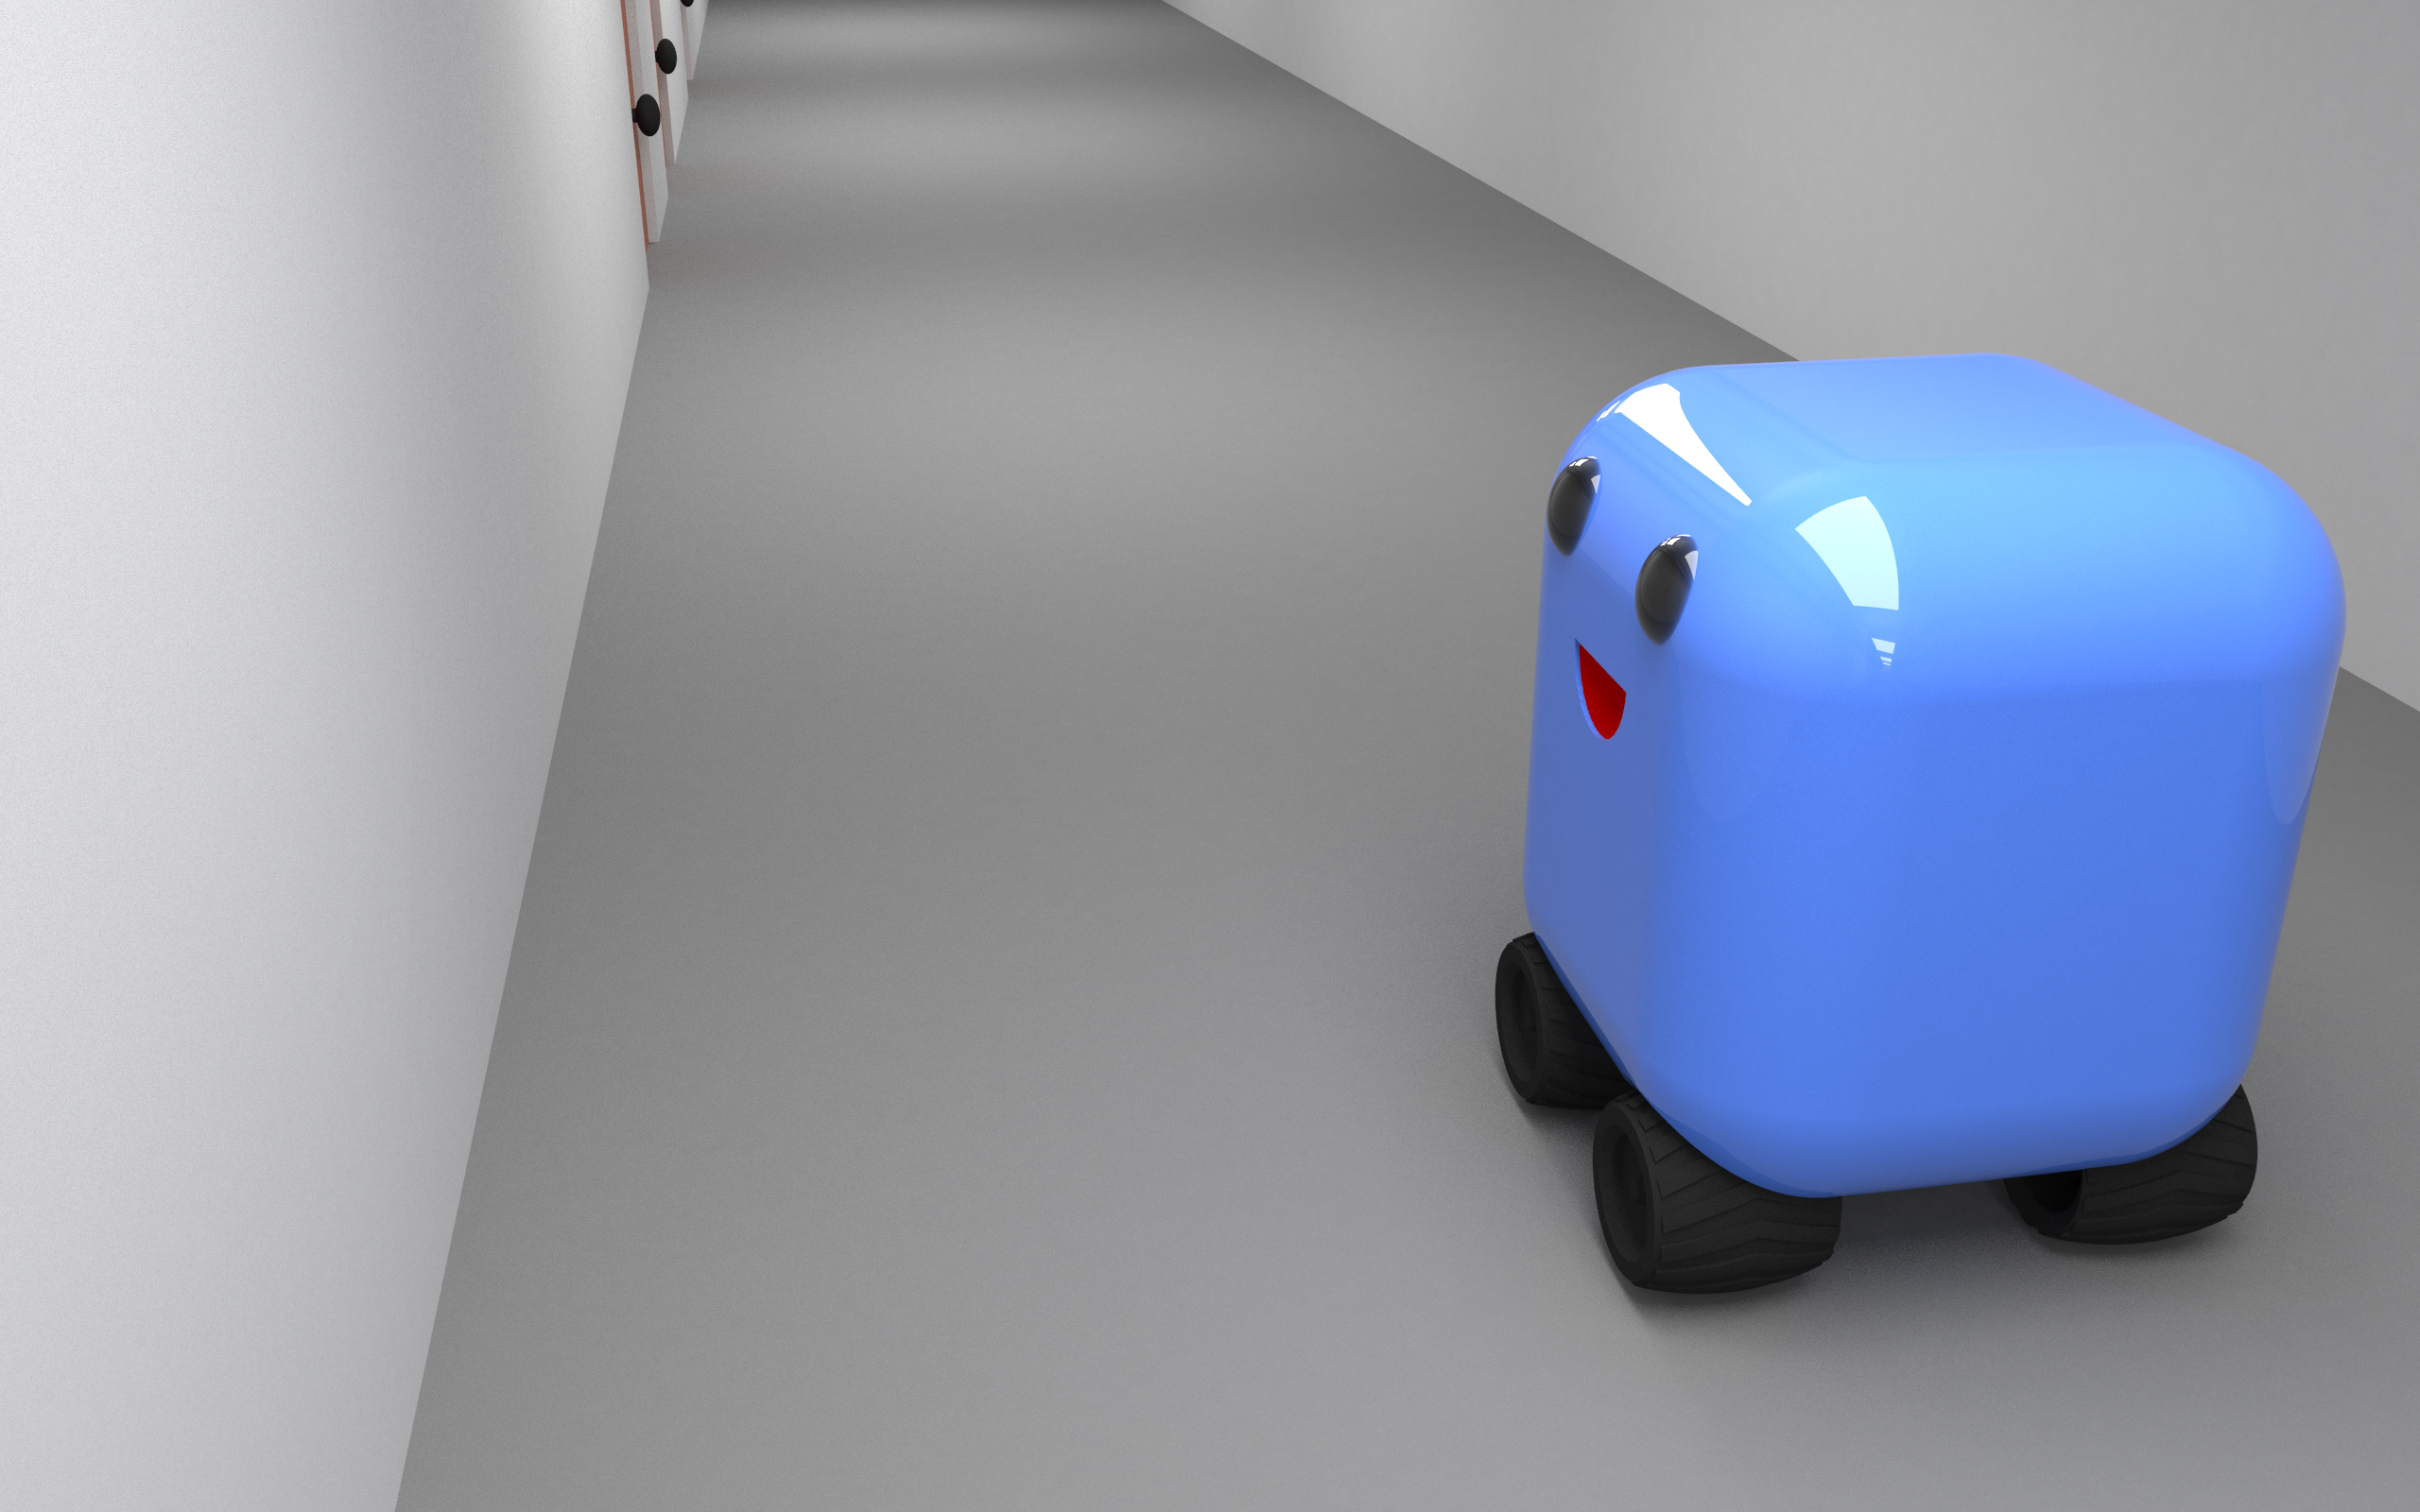
\includegraphics[width=\textwidth]{robotwall.png}
          \caption{La mure et le robot}
          \label{fig:robowall}
        \end{figure}
      \end{block}
    \end{column}
  \end{columns}
\end{frame}

\begin{frame}{Implémentation d'un Agent Simple}
Après la pause de 10 min.
\end{frame}

\end{document}
